\chapter{Introduction}
	\label{chapter:introduction}
	%

\graphicspath{{figures/chapter-1/}}

%=========================================================================

\section{Introduction}

\newglossaryentry{lipsum}{name={lipsum}, description={Lorem Ipsum, a special type of fudge}}
\newglossaryentry{dolor}{name={dolor}, description={No idea why}, parent={lipsum}}
\newglossaryentry{ibit}{name={ibit}, description={Sounds right, doesn't it?}, parent={lipsum}}
\newacronym{dft}{DFT}{density functional theory}
\newglossaryentry{pi}{name={\ensuremath{\pi}}, description={Greek letter pi, \ensuremath{\Pi} does this work?}, symbol={\ensuremath{\pi}}, sort=pi}
\lipsum[1-6]\cite{Narten1967}
\index{a}

\begin{figure}[h]
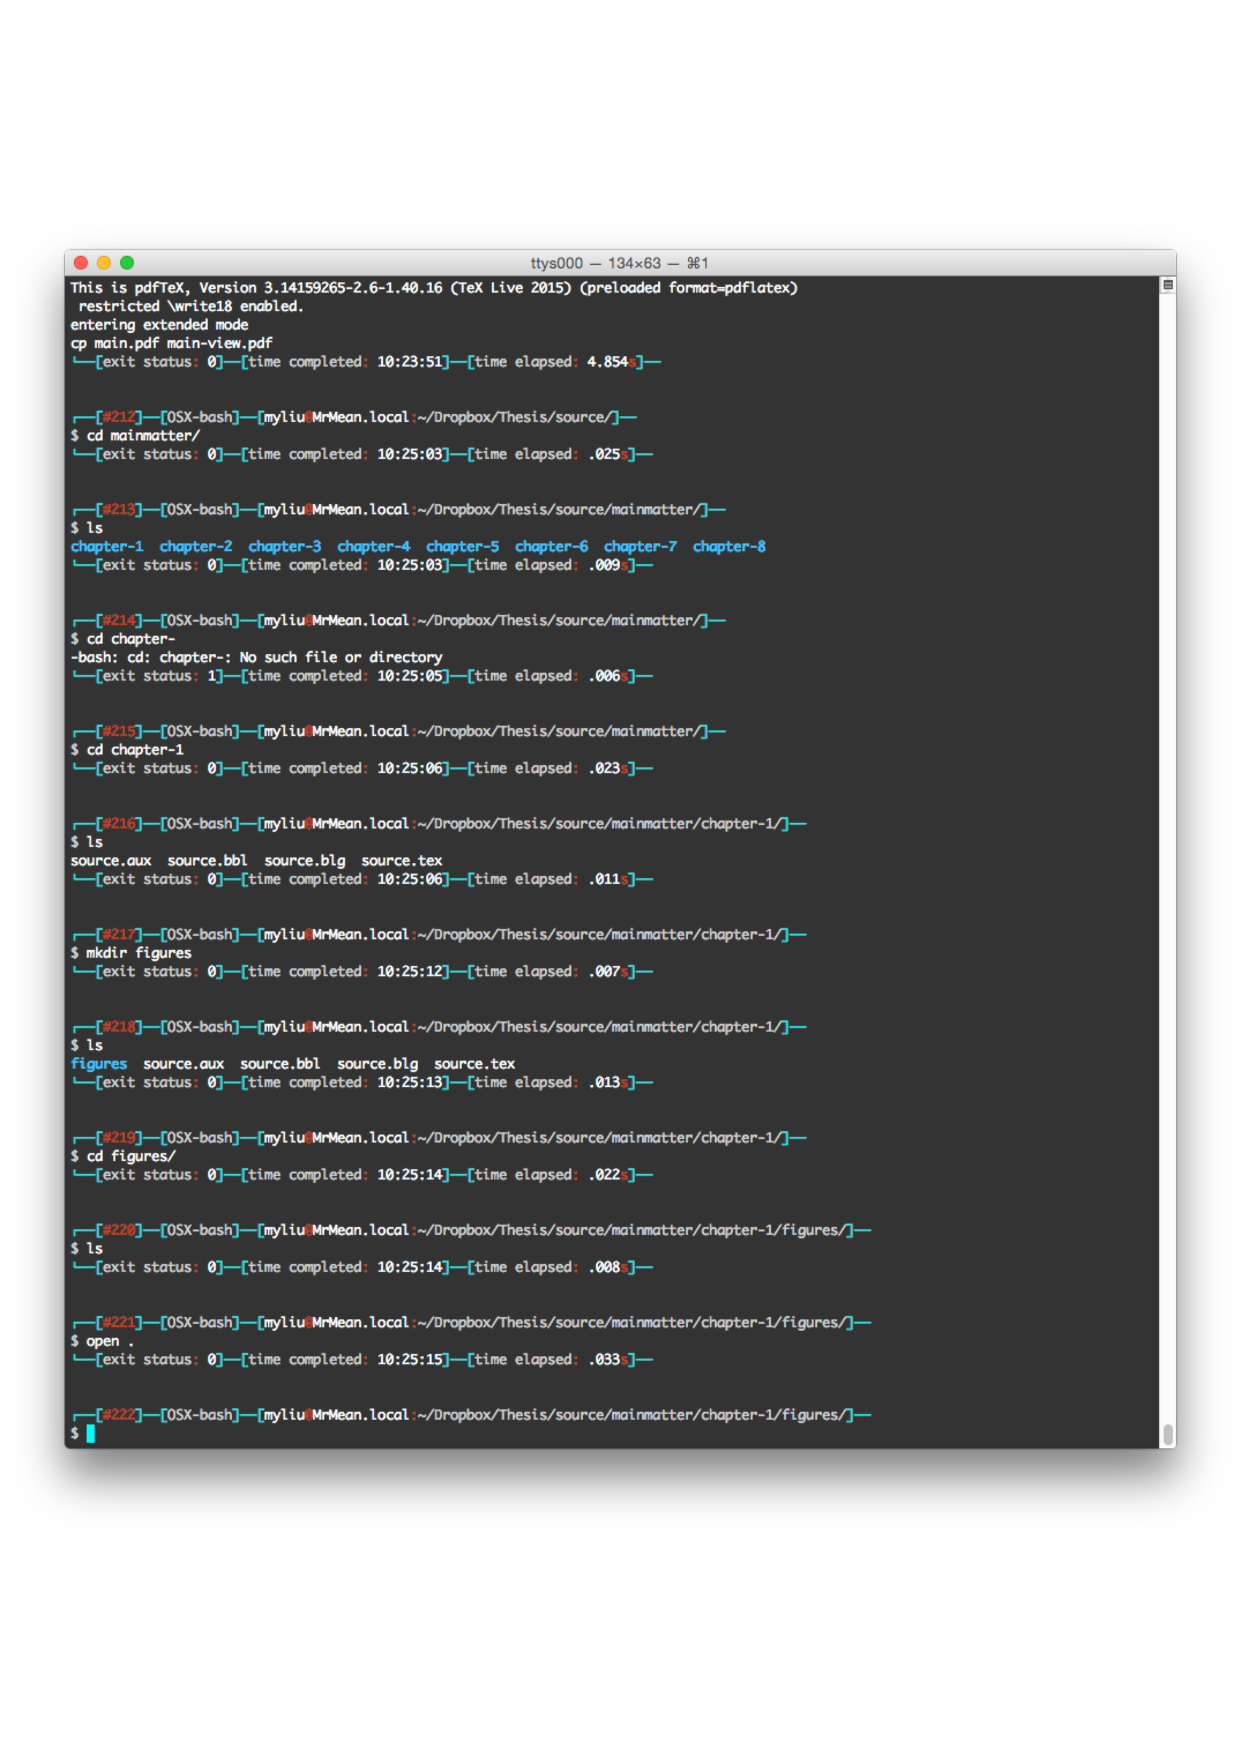
\includegraphics[height=0.7\textheight]{a.pdf}
\caption[This is a short caption]{This is a terminal screen for stuff.\cite{Narten1967}}
\end{figure}

%=========================================================================

\mybib{bib/test.bib}
